
\documentclass[11pt]{article}

% Language setting
\usepackage[turkish]{babel}
\usepackage{pythonhighlight}

\usepackage[a4paper,top=2cm,bottom=2cm,left=2cm,right=2cm,marginparwidth=2cm]{geometry}

% Useful packages
\usepackage{amsmath}
\usepackage{graphicx}
\usepackage[colorlinks=true, allcolors=blue]{hyperref}
\usepackage{verbatim}
\usepackage{fancyhdr} % for header and footer
\usepackage{titlesec}
\usepackage{parskip}

\setlength{\parindent}{0pt}

\titleformat{\subsection}[runin]{\bfseries}{\thesubsection}{1em}{}

\pagestyle{fancy} % activate the custom header/footer

% define the header/footer contents
\lhead{\small{23BLM-4014 Yapay Sinir Ağları Ara Sınav Soru ve Cevap Kağıdı}}
\rhead{\small{Dr. Ulya Bayram}}
\lfoot{}
\rfoot{}

% remove header/footer on first page
\fancypagestyle{firstpage}{
  \lhead{}
  \rhead{}
  \lfoot{}
  \rfoot{\thepage}
}
 

\title{Çanakkale Onsekiz Mart Üniversitesi, Mühendislik Fakültesi, Bilgisayar Mühendisliği Akademik Dönem 2022-2023\\
Ders: BLM-4014 Yapay Sinir Ağları/Bahar Dönemi\\ 
ARA SINAV SORU VE CEVAP KAĞIDI\\
Dersi Veren Öğretim Elemanı: Dr. Öğretim Üyesi Ulya Bayram}
\author{%
\begin{minipage}{\textwidth}
\raggedright
Öğrenci Adı Soyadı: Melis Hürkan\\ % Adınızı soyadınızı ve öğrenci numaranızı noktaların yerine yazın
Öğrenci No: 190401079
\end{minipage}%
}

\date{14 Nisan 2023}

\begin{document}
\maketitle

\vspace{-.5in}
\section*{Açıklamalar:}
\begin{itemize}
    \item Vizeyi çözüp, üzerinde aynı sorular, sizin cevaplar ve sonuçlar olan versiyonunu bu formatta PDF olarak, Teams üzerinden açtığım assignment kısmına yüklemeniz gerekiyor. Bu bahsi geçen PDF'i oluşturmak için LaTeX kullandıysanız, tex dosyasının da yer aldığı Github linkini de ödevin en başına (aşağı url olarak) eklerseniz bonus 5 Puan! (Tavsiye: Overleaf)
    \item Çözümlerde ya da çözümlerin kontrolünü yapmada internetten faydalanmak, ChatGPT gibi servisleri kullanmak serbest. Fakat, herkesin çözümü kendi emeğinden oluşmak zorunda. Çözümlerinizi, cevaplarınızı aşağıda belirttiğim tarih ve saate kadar kimseyle paylaşmayınız. 
    \item Kopyayı önlemek için Github repository'lerinizin hiçbirini \textbf{14 Nisan 2023, saat 15:00'a kadar halka açık (public) yapmayınız!} (Assignment son yükleme saati 13:00 ama internet bağlantısı sorunları olabilir diye en fazla ekstra 2 saat daha vaktiniz var. \textbf{Fakat 13:00 - 15:00 arası yüklemelerden -5 puan!}
    \item Ek puan almak için sağlayacağınız tüm Github repository'lerini \textbf{en geç 15 Nisan 2023 15:00'da halka açık (public) yapmış olun linklerden puan alabilmek için!}
    \item \textbf{14 Nisan 2023, saat 15:00'dan sonra gönderilen vizeler değerlendirilmeye alınmayacak, vize notu olarak 0 (sıfır) verilecektir!} Son anda internet bağlantısı gibi sebeplerden sıfır almayı önlemek için assignment kısmından ara ara çözümlerinizi yükleyebilirsiniz yedekleme için. Verilen son tarih/saatte (14 Nisan 2023, saat 15:00) sistemdeki en son yüklü PDF geçerli olacak.
    \item Çözümlerin ve kodların size ait ve özgün olup olmadığını kontrol eden bir algoritma kullanılacaktır. Kopya çektiği belirlenen vizeler otomatikman 0 (sıfır) alacaktır. Bu nedenle çözümlerinizi ve kodlarınızı yukarıda sağladığım gün ve saatlere kadar kimseyle paylaşmayınız.
    \item Bu vizeden alınabilecek en yüksek not 100'dür. Toplam aldığınız puan 100'ü geçerse, aldığınız not 100'e sabitlenecektir.
    \item LaTeX kullanarak PDF oluşturanlar öz geçmişlerine LaTeX bildiklerini de eklemeyi unutmasınlar :)
    \item Bu vizedeki soruların çözümleri ve tex dosyası için istediğiniz kadar sayıda Github repository'si oluşturabilirsiniz. Sadece yukarıda belirttiğim tarihlerde (14 Nisan 2023 saat 15:00 ile 15 Nisan 2023 saat 15:00 arasında) public yapmayı/halka açmayı ve Github profilinizi de öz geçmişinize eklemeyi unutmayın :)
    \item Bilgisayarınıza hiçbir program kurmadan, Overleaf, Google Colab, Kaggle gibi ortamlar üzerinden bu vizeyi tamamlamanız mümkün. İyi çalışmalar!!
\end{itemize}

(Ekstra 5 puan) \url{https://github.com/melishurkan/OdevTex}

\newpage
\section{(Toplam 10 Puan) Hopfield Networks:}

\subsection{(2 Puan)} \textbf{ChatGPT’ye size Hopfield Network’ler ile ilgili detaylı bilgi vermesini isteyin. Sorduğunuz soruyu, ChatGPT'nin çıkartığı cevabı aşağı koyun. Bu cevapta anlamadığınız terimleri de ChatGPT’ye sorup, sorduğunuz soruları ve ChatGPT’nin verdiği cevapları da sırayla aşağı koyun.}

Hopfield Network tanımı nedir?

Hopfield ağları, yapay sinir ağları sınıfına ait bir modeldir. İsimlerini John Hopfield'dan almışlardır ve aslında bir çeşit enerji tabanlı modeldir. Bu ağlar, birbirleriyle etkileşim halinde olan ve bir dizi işlem yapabilen düğümlerden 
(neuronlar) oluşur.Hopfield ağları, özellikle hatırlama ve optimizasyon problemlerini çözmek için kullanılırlar. Verilen bir problemi, Hopfield ağına uygun şekilde tanımlanmış bir enerji fonksiyonu olarak ifade ederiz ve ağ, 
bu fonksiyonu minimize etmek için çalışır.Ağın belleği, tanımlanan enerji fonksiyonu ile temsil edilir. Bellek, önceden öğrenilmiş örneklerin bir araya getirilmesiyle oluşturulur ve daha sonra, öğrenilmiş bilgileri hatırlamak ve verilen bir girdiyi
 göre hatırlamak için kullanılır.Hopfield ağları, asenkron ve senkron dinamiklerle çalışabilirler. Asenkron dinamiklerde, her bir nöron ayrı ayrı güncellenir, senkron dinamiklerde ise tüm nöronlar aynı anda güncellenir. Hopfield ağları ayrıca,
 her bir düğümün sadece iki olası durumu (0 veya 1) olduğundan, sınırlı bir modeldir.

\subsection{(8 Puan)} \textbf{ChatGPT’nin açıklamalarından ne anladığınızı buraya kendi kelimelerinizle özetleyin. Örneğin ``Hopfield Network nedir? Ne işe yarar? Neden bilmemiz gerekir bunu? Gerçek hayatta kullanılıyor mu?'' gibi. Anlamadığınız kısımlar varsa ve ChatGPT’nin açıklamaları yeterli gelmezse internet dahil farklı kaynaklardan araştırıp, bilgilerin doğruluğunu sorgulamakta serbestsiniz. Konuyu doğru anlayıp anlamamanız puana etki edecektir. Kullandığınız kaynakları da belirtin!}

Özet:Hopfield Ağı, geri beslemeli bir yapay sinir ağıdır ve adını John Hopfield'den almıştır. Bu ağ, aslında bir dizi nöronun birbirine bağlanmasıyla oluşturulur ve her bir nöron diğerlerine bağlıdır. Bu bağlantılar, nöronların birbirleriyle 
etkileşime girerek birbirleriyle etkileşimlerini düzenler.Hopfield ağı, bir dizi giriş öğesinin (inputs) bir desene (pattern) yakın olup olmadığını tanımlamak için kullanılabilir. Bu ağ, bir deseni belleğinde saklar ve daha sonra bu desene benzer
 bir giriş öğesi geldiğinde bu deseni hatırlayabilir. Hopfield ağı, birçok uygulama için kullanılabilir, örneğin veri sıkıştırma ve veri hatası düzeltme gibi.
-Hopefield ağı hangi uygulamalar için kullanılabilir ?
Hopfield ağı, bellek hatırlama, desen tanıma, veri sıkıştırma, veri hatası düzeltme, optik karakter tanıma (OCR), seyahat satıcısı problemini çözme ve daha birçok uygulama için kullanılabilir.
Bellek hatırlama: Hopfield ağı, belleğinde depoladığı desenleri tanıyabilmesi için kullanılabilir. Örneğin, bir ağın belleğinde bir yüzün deseni saklanmışsa, ağ aynı yüzün farklı bir açıdan fotoğrafını aldığında bile bu yüzü tanıyabilir.
Desen tanıma: Hopfield ağı, bir desenin benzerliğini öğrenebilir ve aynı veya benzer desenlerle karşılaştığında tanıyabilir. Örneğin, optik karakter tanıma (OCR) uygulamalarında, hopfield ağı, belirli bir karakterin benzer desenlerini öğrenir ve daha sonra farklı bir görüntüdeki aynı veya benzer karakterleri tanıyabilir.
Veri sıkıştırma: Hopfield ağı, veri sıkıştırma için kullanılabilir. Ağ, bir veri kümesindeki benzer desenleri öğrenir ve daha sonra bu desenlerin bir arada olabileceği şekilde veri setini sıkıştırır.
Veri hatası düzeltme: Hopfield ağı, veri hatası düzeltme için kullanılabilir. Ağ, bir veri setindeki hataları öğrenir ve daha sonra benzer hataları otomatik olarak düzeltir.
Seyahat satıcısı problemi: Hopfield ağı, seyahat satıcısının tüm şehirleri sadece bir kere ziyaret ederek en kısa yolculuk rotasını belirlemesine yardımcı olabilir. Bu problem, birçok uygulamada kullanılabilir, örneğin lojistik yönetimi gibi.
-Hopefield ağı şuan kullanılıyor mu?
Evet, Hopfield ağı hala günümüzde kullanılmaktadır. Özellikle bellek hatırlama ve desen tanıma problemlerinde sıkça kullanılmaktadır. Ayrıca, Hopfield ağı, veri sıkıştırma, 
veri hatası düzeltme ve seyahat satıcısı probleminin çözümünde de kullanılabilir. Bunun yanı sıra, Hopfield ağı, optik karakter tanıma (OCR), işaret tanıma ve ses tanıma gibi birçok alanda kullanılabilir. 
Hopfield ağının günümüzdeki kullanımı, yapay zeka ve makine öğrenimi gibi alanlardaki gelişmeler ile birlikte artmaktadır.
Kaynak :chat gpt

\section{(Toplam 10 Puan) Boltzman Machine:}

\subsection{(2 Puan)} \textbf{ChatGPT’ye size Boltzman Machine ilgili detaylı bilgi vermesini isteyin. Sorduğunuz soruyu, ChatGPT'nin çıkartığı cevabı aşağı koyun. Bu cevapta anlamadığınız terimleri de ChatGPT’ye sorup, sorduğunuz soruları ve ChatGPT’nin verdiği cevapları da sırayla aşağı koyun.}

2-Boltzman Machine nedir ?

Boltzmann Machine, enerji tabanlı bir yapay sinir ağıdır. Bu ağ, stokastik sinir ağları sınıfına aittir ve Belief Propagation (BP) adı verilen bir algoritma ile öğrenir. Boltzmann Machine, içinde birbirleriyle bağlantılı bir dizi gizli ve gözlemci nöronlardan oluşur. 
Ağ,öğrenme sürecinde bağlantıların güncellenmesi yoluyla bir veri setindeki örüntüleri ve ilişkileri öğrenir.
Boltzmann Machine, iki tür nöron içerir: görünür nöronlar ve gizli nöronlar. Görünür nöronlar, ağın girdi verilerinin geldiği yerdir. Gizli nöronlar ise girdi verilerine dayanarak belirlenen öznitelikleri temsil eder.
Ağın her nöronu, bir enerji fonksiyonu tarafından tanımlanır. Bu enerji fonksiyonu, nöronların birbirleriyle olan bağlantılarının toplam etkisini ölçer. Bu etki, sinapslar arasındaki ağırlıklarla belirlenir.
Boltzmann Machine öğrenirken, ağın başlangıçta rastgele başlatılan bağlantı ağırlıkları, enerji fonksiyonu ve bazı diğer parametreler, bir veri setine göre optimize edilir. Bu optimizasyon süreci, genellikle maksimum 
olabilirlik yöntemiyle gerçekleştirilir. Ağın öğrenme süreci, Markov zinciri Monte Carlo (MCMC) gibi yöntemlerle gerçekleştirilir.Boltzmann Machine, birçok uygulama için kullanılabilir. Bunlar arasında örneğin, doğrusal olmayan özellik çıkarımı, 
desen tanıma, öneri sistemleri, veri sıkıştırma, doğrusal olmayan filtreleme ve hatta kuantum hesaplama gibi alanlar yer alır.Boltzmann Machine, ağların derin öğrenmesinde bir dönüm noktası olarak kabul edilir. Bu, ağın temel bir yapı taşı olarak, 
derin öğrenmenin birçok farklı çeşidine ve özellik çıkarımı problemlerinin çözümüne yol açmıştır. Ancak, ağın öğrenme süreci oldukça yavaş olabilir ve bazı uygulamalarda kullanımı zordur. Bu nedenle, Boltzmann Machine genellikle sınırlı kullanıma sahiptir ve daha özel durumlarda kullanılmaktadır.

\subsection{(8 Puan)} \textbf{ChatGPT’nin açıklamalarından ne anladığınızı buraya kendi kelimelerinizle özetleyin. Örneğin ``Boltzman Machine nedir? Ne işe yarar? Neden bilmemiz gerekir bunu? Gerçek hayatta kullanılıyor mu?'' gibi. Anlamadığınız kısımlar varsa ve ChatGPT’nin açıklamaları yeterli gelmezse internet dahil farklı kaynaklardan araştırıp, bilgilerin doğruluğunu sorgulamakta serbestsiniz. Konuyu doğru anlayıp anlamamanız puana etki edecektir. Kullandığınız kaynakları da belirtin!}

özet:Boltzmann makineleri, yapay sinir ağları alanında önemli bir modeldir.
Bu model, yüksek düzeyde paralel işlemler gerçekleştirebilen, olasılık tabanlı bir modeldir.
Bir Boltzmann makinesi, bir veya daha fazla gizli katmanı olan bir yapay sinir ağıdır.
Boltzmann makineleri, veri dağılımlarını modellemek için kullanılır ve birçok uygulama alanında kullanılabilirler.
Bir Boltzmann makinesinin çalışma prensibi, enerji fonksiyonuna dayanır.
Bu fonksiyon, verilen bir girişe göre bir enerji seviyesi üretir.
Daha sonra, sistem rastgele hareket eder ve enerji fonksiyonundaki değişikliklere göre kendini düzenler.
Boltzmann makineleri, hem denetimsiz öğrenme hem de çıktı üretimi için kullanılabilirler.
-Boltzman Makineleri hangi uygulamalarda kullanılıyor ?
Boltzmann makineleri, özellikle veri modellemesi, sınıflandırma ve kümeleme gibi veri analizi görevleri için kullanışlıdırlar. Aşağıda Boltzmann makinelerinin kullanılabileceği bazı uygulama alanları verilmiştir:
Görüntü İşleme: Boltzmann makineleri, görüntü işleme uygulamalarında kullanılabilecek özellik çıkarma ve özellik seçimi için kullanışlıdırlar.
Doğal Dil İşleme: Boltzmann makineleri, doğal dil işleme uygulamalarında kullanılabilecek kelime özellikleri, kelime sırası vb. için kullanılabilirler.
Öneri Sistemleri: Boltzmann makineleri, öneri sistemlerinde kullanılan veri modellemesi için kullanılabilirler.
Anomalilerin Tespiti: Boltzmann makineleri, veri dağılımlarındaki anormallikleri tespit etmek için kullanılabilirler.
Finansal Tahminler: Boltzmann makineleri, finansal tahminler yapmak için kullanılabilecek birçok veri setini modellemek için kullanılabilirler.
Otomatik Veri Kodlama: Boltzmann makineleri, veri setleri için otomatik kodlama yapmak için kullanılabilirler.
Sentiment Analizi: Boltzmann makineleri, metinlerdeki hissiyatı anlamak için kullanılabilirler.
Robotik ve Otonom Araçlar: Boltzmann makineleri, robotik ve otonom araçlarda kullanılan sensör verilerini işlemek için kullanılabilirler.
kaynak : Chat GPT

\section{(Toplam 10 Puan) Markov Assumption ve Markov Chain:}

\subsection{(2 Puan)} \textbf{ChatGPT’ye size Markov assumption ve Markov Chain ilgili detaylı bilgi vermesini isteyin. Sorduğunuz soruyu, ChatGPT'nin çıkartığı cevabı aşağı koyun. Bu cevapta anlamadığınız terimleri de ChatGPT’ye sorup, sorduğunuz soruları ve ChatGPT’nin verdiği cevapları da sırayla aşağı koyun.}

Markov assumption ve Markov Chain nedir?

Markov Assumption, bir sürecin mevcut durumunun, yalnızca son birkaç durumdan ve mevcut durumun bağımsız olarak belirlendiği varsayımına dayanır. Bu varsayım, bir sürecin geçmişinin mevcut durum üzerindeki etkisinin önemsiz olduğunu varsayar.
Markov Zinciri, Markov Assumption'un sağlandığı bir süreçtir. Bir Markov Zinciri, bir dizi olayın sürekli bir şekilde gerçekleştiği bir süreci ifade eder. Bu süreçte, her bir olayın gerçekleşme olasılığı, sadece mevcut durumdan bağımsızdır ve önceki olayların gerçekleşme olasılıklarından etkilenmez. Bir Markov Zinciri'nin her bir durumu, bir "durum uzayı" olarak adlandırılır ve her bir durum, sürecin mevcut durumunu belirler.
Markov Zinciri, iki ana bileşenden oluşur: durum uzayı ve geçiş olasılıkları matrisi. Durum uzayı, Markov Zinciri'nin tüm olası durumlarını ifade ederken, geçiş olasılıkları matrisi, her bir durumun diğer tüm durumlara geçiş olasılıklarını gösterir.
Markov Zinciri, birçok uygulama için önemlidir. Örneğin, finansal piyasalardaki fiyat hareketleri, hava durumu modelleri ve spam filtreleme algoritmaları gibi birçok alanda kullanılır.

\subsection{(8 Puan)} \textbf{ChatGPT’nin açıklamalarından ne anladığınızı buraya kendi kelimelerinizle özetleyin. Örneğin ``Markov assumption ve Markov Chain nedir? Ne işe yarar? Neden bilmemiz gerekir bunu? Gerçek hayatta kullanılıyor mu?'' gibi. Anlamadığınız kısımlar varsa ve ChatGPT’nin açıklamaları yeterli gelmezse internet dahil farklı kaynaklardan araştırıp, bilgilerin doğruluğunu sorgulamakta serbestsiniz. Konuyu doğru anlayıp anlamamanız puana etki edecektir. Kullandığınız kaynakları da belirtin!}

Markov assumption ne işe yarar ?

Markov Assumption, özellikle zaman serileri analizi, sinyal işleme, optimizasyon ve yapay zeka gibi birçok alanda önemli bir rol oynar. 
Bu varsayım, daha önceki durumların kaydedilmesi veya takip edilmesi gerekmeksizin gelecekteki durumların tahmin edilmesini kolaylaştırır.
Örneğin, finansal piyasalardaki fiyat hareketleri, hava durumu modelleri ve spam filtreleme algoritmaları gibi birçok alanda Markov Zinciri ve Markov Assumption kullanılır. 
Bu algoritmalar, geçmiş verilerin kullanımını azaltarak gelecekteki durumları daha hızlı ve doğru bir şekilde tahmin etmeye yardımcı olur.

Markov Chain Nedir ?

Markov zinciri, önceki olayların sonraki olaylar üzerindeki etkisini modellemek için kullanılan bir matematiksel modeldir. Bu model, bir sistemdeki durumları ve bu durumlar arasındaki geçişlerin olasılıklarını temsil eder.
Markov zincirleri, birçok alanda kullanılır. Örneğin, finansal piyasaların analizi, meteorolojik modeller, doğal dil işleme ve makine öğrenmesi gibi alanlarda kullanılır.
Finansal piyasaların analizinde, Markov zincirleri genellikle fiyatların hareketini modeller. Bu, geçmiş fiyatların, gelecekteki fiyatların olasılıklı hareketlerine işaret eden bir model oluşturmak için kullanılır.
Meteorolojik modellerde, Markov zincirleri, mevcut hava durumu durumunun sonraki hava durumunu etkilediği gerçeğini kullanarak hava durumu tahminlerinde kullanılır.
Doğal dil işlemede, Markov zincirleri, metindeki kelimeler arasındaki olasılıklı ilişkileri modellemek için kullanılır.
Makine öğrenmesinde, Markov zincirleri, bir sınıflandırma problemi çözmek için kullanılabilir. Bu durumda, bir nesnenin sınıfı,
o nesnenin özelliklerine ve sınıfını tahmin etmek için kullanılan önceki nesnelerin sınıflarına dayanarak belirlenir.

Özet:

Markov Assumption, bir sürecin mevcut durumunun, yalnızca son birkaç durumdan ve mevcut durumun bağımsız olarak belirlendiği varsayımına dayanır.
Bu varsayım, bir sürecin geçmişinin mevcut durum üzerindeki etkisinin önemsiz olduğunu varsayar.
Bir Markov Zinciri, bir dizi olayın sürekli bir şekilde gerçekleştiği bir süreci ifade eder.
Bir Markov Zinciri'nin her bir durumu, bir ‘‘durum uzayı‘‘ olarak adlandırılır ve her bir durum, sürecin mevcut durumunu belirler.
Markov Zinciri, iki ana bileşenden oluşur: durum uzayı ve geçiş olasılıkları matrisi.
Durum uzayı, Markov Zinciri'nin tüm olası durumlarını ifade ederken, geçiş olasılıkları matrisi, her bir durumun diğer tüm durumlara geçiş olasılıklarını gösterir.
Markov Zinciri, birçok uygulama için önemlidir.

\section{(Toplam 20 Puan) Feed Forward:}
 
\begin{itemize}
    \item Forward propagation için, input olarak şu X matrisini verin (tensöre çevirmeyi unutmayın):\\
    $X = \begin{bmatrix}
        1 & 2 & 3\\
        4 & 5 & 6
        \end{bmatrix}$
    Satırlar veriler (sample'lar), kolonlar öznitelikler (feature'lar).
    \item Bir adet hidden layer olsun ve içinde tanh aktivasyon fonksiyonu olsun
    \item Hidden layer'da 50 nöron olsun
    \item Bir adet output layer olsun, tek nöronu olsun ve içinde sigmoid aktivasyon fonksiyonu olsun
\end{itemize}

Tanh fonksiyonu:\\
$f(x) = \frac{exp(x) - exp(-x)}{exp(x) + exp(-x)}$
\vspace{.2in}

Sigmoid fonksiyonu:\\
$f(x) = \frac{1}{1 + exp(-x)}$

\vspace{.2in}
 \textbf{Pytorch kütüphanesi ile, ama kütüphanenin hazır aktivasyon fonksiyonlarını kullanmadan, formülünü verdiğim iki aktivasyon fonksiyonunun kodunu ikinci haftada yaptığımız gibi kendiniz yazarak bu yapay sinir ağını oluşturun ve aşağıdaki üç soruya cevap verin.}
 
\subsection{(10 Puan)} \textbf{Yukarıdaki yapay sinir ağını çalıştırmadan önce pytorch için Seed değerini 1 olarak set edin, kodu aşağıdaki kod bloğuna ve altına da sonucu yapıştırın:}

% Latex'de kod koyabilirsiniz python formatında. Aşağıdaki örnekleri silip içine kendi kodunuzu koyun
\begin{python}
import numpy as np
import torch


np.random.seed(1)

X = np.array([[1, 2, 3], [4, 5, 6]])


input_size = X.shape[1]  
hidden_size = 50          
output_size = 1           

W1 = np.random.randn(input_size, hidden_size)  
b1 = np.zeros((1, hidden_size))               
W2 = np.random.randn(hidden_size, output_size) 
b2 = np.zeros((1, output_size))               


def tanh(x):
    return (torch.exp(torch.tensor(x)) - torch.exp(torch.tensor(-x))) / (torch.exp(torch.tensor(x)) + torch.exp(torch.tensor(-x)))


def sigmoid(x):
    return 1 / (1 + np.exp(-x))


z1 = np.dot(X, W1) + b1   
a1 = tanh(z1)            
z2 = np.dot(a1, W2) + b2  
y_pred = torch.tensor(sigmoid(z2)) 

print(y_pred)
\end{python}

tensor([[0.9999],
        [0.9997]])

\subsection{(5 Puan)} \textbf{Yukarıdaki yapay sinir ağını çalıştırmadan önce Seed değerini öğrenci numaranız olarak değiştirip, kodu aşağıdaki kod bloğuna ve altına da sonucu yapıştırın:}

\begin{python}
import numpy as np
import torch


np.random.seed(190401079)

X = np.array([[1, 2, 3], [4, 5, 6]])


input_size = X.shape[1]  
hidden_size = 50          
output_size = 1           

W1 = np.random.randn(input_size, hidden_size)  
b1 = np.zeros((1, hidden_size))               
W2 = np.random.randn(hidden_size, output_size) 
b2 = np.zeros((1, output_size))               


def tanh(x):
    return (torch.exp(torch.tensor(x)) - torch.exp(torch.tensor(-x))) / (torch.exp(torch.tensor(x)) + torch.exp(torch.tensor(-x)))


def sigmoid(x):
    return 1 / (1 + np.exp(-x))


z1 = np.dot(X, W1) + b1   
a1 = tanh(z1)            
z2 = np.dot(a1, W2) + b2  
y_pred = torch.tensor(sigmoid(z2)) 

print(y_pred)
\end{python}

tensor([[0.8982],
        [0.9556]])

\subsection{(5 Puan)} \textbf{Kodlarınızın ve sonuçlarınızın olduğu jupyter notebook'un Github repository'sindeki linkini aşağıdaki url kısmının içine yapıştırın. İlk sayfada belirttiğim gün ve saate kadar halka açık (public) olmasın:}
% size ait Github olmak zorunda, bu vize için ayrı bir github repository'si açıp notebook'u onun içine koyun. Kendine ait olmayıp da arkadaşının notebook'unun linkini paylaşanlar 0 alacak.

\url{https://github.com/melishurkan/Soru4}

\section{(Toplam 40 Puan) Multilayer Perceptron (MLP):} 
\textbf{Bu bölümdeki sorularda benim vize ile beraber paylaştığım Prensesi İyileştir (Cure The Princess) Veri Seti parçaları kullanılacak. Hikaye şöyle (soruyu çözmek için hikaye kısmını okumak zorunda değilsiniz):} 

``Bir zamanlar, çok uzaklarda bir ülkede, ağır bir hastalığa yakalanmış bir prenses yaşarmış. Ülkenin kralı ve kraliçesi onu iyileştirmek için ellerinden gelen her şeyi yapmışlar, ancak denedikleri hiçbir çare işe yaramamış.

Yerel bir grup köylü, herhangi bir hastalığı iyileştirmek için gücü olduğu söylenen bir dizi sihirli malzemeden bahsederek kral ve kraliçeye yaklaşmış. Ancak, köylüler kral ile kraliçeyi, bu malzemelerin etkilerinin patlayıcı olabileceği ve son zamanlarda yaşanan kuraklıklar nedeniyle bu malzemelerden sadece birkaçının herhangi bir zamanda bulunabileceği konusunda uyarmışlar. Ayrıca, sadece deneyimli bir simyacı bu özelliklere sahip patlayıcı ve az bulunan malzemelerin belirli bir kombinasyonunun prensesi iyileştireceğini belirleyebilecekmiş.

Kral ve kraliçe kızlarını kurtarmak için umutsuzlar, bu yüzden ülkedeki en iyi simyacıyı bulmak için yola çıkmışlar. Dağları tepeleri aşmışlar ve nihayet "Yapay Sinir Ağları Uzmanı" olarak bilinen yeni bir sihirli sanatın ustası olarak ün yapmış bir simyacı bulmuşlar.

Simyacı önce köylülerin iddialarını ve her bir malzemenin alınan miktarlarını, ayrıca iyileşmeye yol açıp açmadığını incelemiş. Simyacı biliyormuş ki bu prensesi iyileştirmek için tek bir şansı varmış ve bunu doğru yapmak zorundaymış. (Original source: \url{https://www.kaggle.com/datasets/unmoved/cure-the-princess})

(Buradan itibaren ChatGPT ve Dr. Ulya Bayram'a ait hikayenin devamı)

Simyacı, büyülü bileşenlerin farklı kombinasyonlarını analiz etmek ve denemek için günler harcamış. Sonunda birkaç denemenin ardından prensesi iyileştirecek çeşitli karışım kombinasyonları bulmuş ve bunları bir veri setinde toplamış. Daha sonra bu veri setini eğitim, validasyon ve test setleri olarak üç parçaya ayırmış ve bunun üzerinde bir yapay sinir ağı eğiterek kendi yöntemi ile prensesi iyileştirme ihtimalini hesaplamış ve ikna olunca kral ve kraliçeye haber vermiş. Heyecanlı ve umutlu olan kral ve kraliçe, simyacının prensese hazırladığı ilacı vermesine izin vermiş ve ilaç işe yaramış ve prenses hastalığından kurtulmuş.

Kral ve kraliçe, kızlarının hayatını kurtardığı için simyacıya krallıkta kalması ve çalışmalarına devam etmesi için büyük bir araştırma bütçesi ve çok sayıda GPU'su olan bir server vermiş. İyileşen prenses de kendisini iyileştiren yöntemleri öğrenmeye merak salıp, krallıktaki üniversitenin bilgisayar mühendisliği bölümüne girmiş ve mezun olur olmaz da simyacının yanında, onun araştırma grubunda çalışmaya başlamış. Uzun yıllar birlikte krallıktaki insanlara, hayvanlara ve doğaya faydalı olacak yazılımlar geliştirmişler, ve simyacı emekli olduğunda prenses hem araştırma grubunun hem de krallığın lideri olarak hayatına devam etmiş.

Prenses, kendisini iyileştiren veri setini de, gelecekte onların izinden gidecek bilgisayar mühendisi prensler ve prensesler başkalarına faydalı olabilecek yapay sinir ağları oluşturmayı öğrensinler diye halka açmış ve sınavlarda kullanılmasını salık vermiş.''

\textbf{İki hidden layer'lı bir Multilayer Perceptron (MLP) oluşturun beşinci ve altıncı haftalarda yaptığımız gibi. Hazır aktivasyon fonksiyonlarını kullanmak serbest. İlk hidden layer'da 100, ikinci hidden layer'da 50 nöron olsun. Hidden layer'larda ReLU, output layer'da sigmoid aktivasyonu olsun.}

\textbf{Output layer'da kaç nöron olacağını veri setinden bakıp bulacaksınız. Elbette bu veriye uygun Cross Entropy loss yöntemini uygulayacaksınız. Optimizasyon için Stochastic Gradient Descent yeterli. Epoch sayınızı ve learning rate'i validasyon seti üzerinde denemeler yaparak (loss'lara overfit var mı diye bakarak) kendiniz belirleyeceksiniz. Batch size'ı 16 seçebilirsiniz.}

\subsection{(10 Puan)} \textbf{Bu MLP'nin pytorch ile yazılmış class'ının kodunu aşağı kod bloğuna yapıştırın:}

\begin{python}



import torch
import torch.nn as nn
import torch.optim as optim
import pandas as pd
import matplotlib.pyplot as plt
class MLP(nn.Module):
    def __init__(self):
        super().__init__()
        self.hidden1 = nn.Linear(13, 100)
        self.hidden2 = nn.Linear(100, 50)
        self.out = nn.Linear(50, 1)

    def forward(self, x):
        x = torch.relu(self.hidden1(x))
        x = torch.relu(self.hidden2(x))
        x = torch.sigmoid(self.out(x))
        return x
\end{python}

\subsection{(10 Puan)} \textbf{SEED=öğrenci numaranız set ettikten sonra altıncı haftada yazdığımız gibi training batch'lerinden eğitim loss'ları, validation batch'lerinden validasyon loss değerlerini hesaplayan kodu aşağıdaki kod bloğuna yapıştırın ve çıkan figürü de alta ekleyin.}

\begin{python}
import torch
import torch.nn as nn
import torch.optim as optim
import pandas as pd
import matplotlib.pyplot as plt


train_data = pd.read_csv("sample_data/cure_the_princess_train.csv")
test_data = pd.read_csv("sample_data/cure_the_princess_test.csv")
val_data = pd.read_csv("sample_data/cure_the_princess_validation.csv")


train_inputs = torch.tensor(train_data.drop("Cured", axis=1).values, dtype=torch.float32)
train_targets = torch.tensor(train_data["Cured"].values, dtype=torch.float32)
test_inputs = torch.tensor(test_data.drop("Cured", axis=1).values, dtype=torch.float32)
test_targets = torch.tensor(test_data["Cured"].values, dtype=torch.float32)
val_inputs = torch.tensor(val_data.drop("Cured", axis=1).values, dtype=torch.float32)
val_targets = torch.tensor(val_data["Cured"].values, dtype=torch.float32)


class MLP(nn.Module):
    def __init__(self):
        super().__init__()
        self.hidden1 = nn.Linear(13, 100)
        self.hidden2 = nn.Linear(100, 50)
        self.out = nn.Linear(50, 1)

    def forward(self, x):
        x = torch.relu(self.hidden1(x))
        x = torch.relu(self.hidden2(x))
        x = torch.sigmoid(self.out(x))
        return x


model = MLP()
optimizer = optim.SGD(model.parameters(), lr=0.01)
criterion = nn.BCELoss()
torch.manual_seed(190401079)


train_losses, val_losses = [], []
num_epochs = 1000
batch_size = 16

for epoch in range(num_epochs):
    for i in range(0, len(train_inputs), batch_size):
        batch_inputs = train_inputs[i:i+batch_size]
        batch_targets = train_targets[i:i+batch_size]

        optimizer.zero_grad()
        outputs = model(batch_inputs).squeeze()
        loss = criterion(outputs, batch_targets)
        loss.backward()
        optimizer.step()

    
    with torch.no_grad():
        train_outputs = model(train_inputs).squeeze()
        train_loss = criterion(train_outputs, train_targets)
        train_losses.append(train_loss.item())

        val_outputs = model(val_inputs).squeeze()
        val_loss = criterion(val_outputs, val_targets)
        val_losses.append(val_loss.item())

        train_predictions = (model(train_inputs) > 0.5).float()
        test_predictions = (model(test_inputs) > 0.5).float()
        val_predictions = (model(val_inputs) > 0.5).float()

    
    if epoch > 10 and val_losses[-1] > val_losses[-3]:
        break

    
    if epoch % 1 == 0:
        print(f"Epoch {epoch} | Train Loss: {train_loss:.5f} | Val Loss: {val_loss:.5f}")



test_outputs = model(test_inputs).squeeze()
test_loss = criterion(test_outputs, test_targets)
test_acc = ((test_outputs > 0.5).float() == test_targets).float().mean()

print(f"Test Loss: {test_loss:.5f} | Test Acc: {test_acc:.5f}")

plt.plot(train_losses, label="Train Loss")
plt.plot(val_losses, label="Val Loss")
plt.legend()
plt.show()
\end{python}

% Figure aşağıda comment içindeki kısımdaki gibi eklenir.

\begin{figure}[ht!]
    \centering
    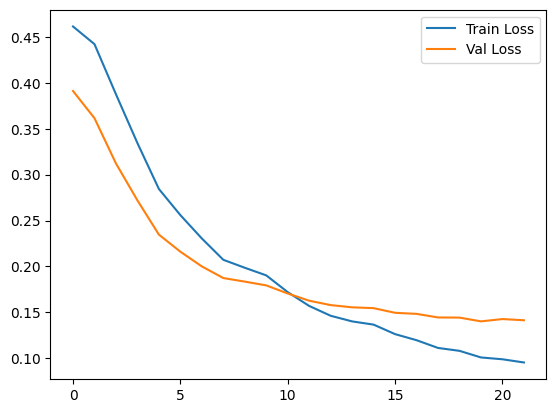
\includegraphics[width=0.75\textwidth]{resim1.png}
    \caption{Train ve Validation kayıp değerlerini gösteren grafik}
    \label{fig:my_pic}
\end{figure}
\newpage

\subsection{(10 Puan)} \textbf{SEED=öğrenci numaranız set ettikten sonra altıncı haftada ödev olarak verdiğim gibi earlystopping'deki en iyi modeli kullanarak, Prensesi İyileştir test setinden accuracy, F1, precision ve recall değerlerini hesaplayan kodu yazın ve sonucu da aşağı yapıştırın. \%80'den fazla başarı bekliyorum test setinden. Daha düşükse başarı oranınız, nerede hata yaptığınızı bulmaya çalışın. \%90'dan fazla başarı almak mümkün (ben denedim).}

\begin{python}
#5.1 

import torch
import torch.nn as nn
import torch.optim as optim
import pandas as pd
import matplotlib.pyplot as plt


train_data = pd.read_csv("sample_data/cure_the_princess_train.csv")
test_data = pd.read_csv("sample_data/cure_the_princess_test.csv")
val_data = pd.read_csv("sample_data/cure_the_princess_validation.csv")


train_inputs = torch.tensor(train_data.drop("Cured", axis=1).values, dtype=torch.float32)
train_targets = torch.tensor(train_data["Cured"].values, dtype=torch.float32)
test_inputs = torch.tensor(test_data.drop("Cured", axis=1).values, dtype=torch.float32)
test_targets = torch.tensor(test_data["Cured"].values, dtype=torch.float32)
val_inputs = torch.tensor(val_data.drop("Cured", axis=1).values, dtype=torch.float32)
val_targets = torch.tensor(val_data["Cured"].values, dtype=torch.float32)


class MLP(nn.Module):
    def __init__(self):
        super().__init__()
        self.hidden1 = nn.Linear(13, 100)
        self.hidden2 = nn.Linear(100, 50)
        self.out = nn.Linear(50, 1)

    def forward(self, x):
        x = torch.relu(self.hidden1(x))
        x = torch.relu(self.hidden2(x))
        x = torch.sigmoid(self.out(x))
        return x


model = MLP()
optimizer = optim.SGD(model.parameters(), lr=0.01)
criterion = nn.BCELoss()
torch.manual_seed(190401079)


train_losses, val_losses = [], []
num_epochs = 1000
batch_size = 16

for epoch in range(num_epochs):
    for i in range(0, len(train_inputs), batch_size):
        batch_inputs = train_inputs[i:i+batch_size]
        batch_targets = train_targets[i:i+batch_size]

        optimizer.zero_grad()
        outputs = model(batch_inputs).squeeze()
        loss = criterion(outputs, batch_targets)
        loss.backward()
        optimizer.step()

    
    with torch.no_grad():
        train_outputs = model(train_inputs).squeeze()
        train_loss = criterion(train_outputs, train_targets)
        train_losses.append(train_loss.item())

        val_outputs = model(val_inputs).squeeze()
        val_loss = criterion(val_outputs, val_targets)
        val_losses.append(val_loss.item())

        train_predictions = (model(train_inputs) > 0.5).float()
        test_predictions = (model(test_inputs) > 0.5).float()
        val_predictions = (model(val_inputs) > 0.5).float()

    
    if epoch > 10 and val_losses[-1] > val_losses[-3]:
        break

    
    if epoch % 1 == 0:
        print(f"Epoch {epoch} | Train Loss: {train_loss:.5f} | Val Loss: {val_loss:.5f}")



test_outputs = model(test_inputs).squeeze()
test_loss = criterion(test_outputs, test_targets)
test_acc = ((test_outputs > 0.5).float() == test_targets).float().mean()

print(f"Test Loss: {test_loss:.5f} | Test Acc: {test_acc:.5f}")

plt.plot(train_losses, label="Train Loss")
plt.plot(val_losses, label="Val Loss")
plt.legend()
plt.show()


from sklearn.metrics import f1_score, accuracy_score, recall_score, precision_score

train_f1 = f1_score(train_targets, train_predictions)
train_acc = accuracy_score(train_targets, train_predictions)
train_recall = recall_score(train_targets, train_predictions)
train_precision = precision_score(train_targets, train_predictions)

test_f1 = f1_score(test_targets, test_predictions)
test_acc = accuracy_score(test_targets, test_predictions)
test_recall = recall_score(test_targets, test_predictions)
test_precision = precision_score(test_targets, test_predictions)

val_f1 = f1_score(val_targets, val_predictions)
val_acc = accuracy_score(val_targets, val_predictions)
val_recall = recall_score(val_targets, val_predictions)
val_precision = precision_score(val_targets, val_predictions)


print("Train:")
print(f"F1 Score: {train_f1:.5f} | Accuracy: {train_acc:.5f} | Recall: {train_recall:.5f} | Precision: {train_precision:.5f}")
print("Test:")
print(f"F1 Score: {test_f1:.5f} | Accuracy: {test_acc:.5f} | Recall: {test_recall:.5f} | Precision: {test_precision:.5f}")
print("Val:")
print(f"F1 Score: {val_f1:.5f} | Accuracy: {val_acc:.5f} | Recall: {val_recall:.5f} | Precision: {val_precision:.5f}")

\end{python}

Epoch 0 | Train Loss: 0.46138 | Val Loss: 0.39113

Epoch 1 | Train Loss: 0.44212 | Val Loss: 0.36147

Epoch 2 | Train Loss: 0.38754 | Val Loss: 0.31217

Epoch 3 | Train Loss: 0.33433 | Val Loss: 0.27196

Epoch 4 | Train Loss: 0.28436 | Val Loss: 0.23466

Epoch 5 | Train Loss: 0.25590 | Val Loss: 0.21608

Epoch 6 | Train Loss: 0.23046 | Val Loss: 0.20004

Epoch 7 | Train Loss: 0.20724 | Val Loss: 0.18737

Epoch 8 | Train Loss: 0.19857 | Val Loss: 0.18347

Epoch 9 | Train Loss: 0.19026 | Val Loss: 0.17937

Epoch 10 | Train Loss: 0.17200 | Val Loss: 0.17054

Epoch 11 | Train Loss: 0.15697 | Val Loss: 0.16268

Epoch 12 | Train Loss: 0.14627 | Val Loss: 0.15790

Epoch 13 | Train Loss: 0.14014 | Val Loss: 0.15547

Epoch 14 | Train Loss: 0.13662 | Val Loss: 0.15457

Epoch 15 | Train Loss: 0.12628 | Val Loss: 0.14950

Epoch 16 | Train Loss: 0.11966 | Val Loss: 0.14835

Epoch 17 | Train Loss: 0.11123 | Val Loss: 0.14444

Epoch 18 | Train Loss: 0.10806 | Val Loss: 0.14429

Epoch 19 | Train Loss: 0.10087 | Val Loss: 0.14018

Epoch 20 | Train Loss: 0.09889 | Val Loss: 0.14269

Test Loss: 0.14194 | Test Acc: 0.94689

Train:F1 Score: 0.96862 | Accuracy: 0.96885 | Recall: 0.97569 | Precision: 0.96166

Test:F1 Score: 0.94641 | Accuracy: 0.94689 | Recall: 0.93299 | Precision: 0.96021

Val:F1 Score: 0.95268 | Accuracy: 0.95223 | Recall: 0.96795 | Precision: 0.93789

\subsection{(5 Puan)} \textbf{Tüm kodların CPU'da çalışması ne kadar sürüyor hesaplayın. Sonra to device yöntemini kullanarak modeli ve verileri GPU'ya atıp kodu bir de böyle çalıştırın ve ne kadar sürdüğünü hesaplayın. Süreleri aşağıdaki tabloya koyun. GPU için Google Colab ya da Kaggle'ı kullanabilirsiniz, iki ortam da her hafta saatlerce GPU hakkı veriyor.}

\begin{table}[ht!]
    \centering
    \caption{Buraya bir açıklama yazın}
    \begin{tabular}{c|c}
        Ortam & Süre (saniye) \\\hline
        CPU & 4.540311813354492 saniye \\
        GPU & 1.6654999256134033 saniye\\
    \end{tabular}
    \label{tab:my_table}
\end{table}

\subsection{(3 Puan)} \textbf{Modelin eğitim setine overfit etmesi için elinizden geldiği kadar kodu gereken şekilde değiştirin, validasyon loss'unun açıkça yükselmeye başladığı, training ve validation loss'ları içeren figürü aşağı koyun ve overfit için yaptığınız değişiklikleri aşağı yazın. Overfit, tam bir çanak gibi olmalı ve yükselmeli. Ona göre parametrelerle oynayın.}

Batch size 16 değerini 10 yaptım ve o şekilde gözlemledim.

% Figür aşağı

\begin{figure}[ht!]
    \centering
    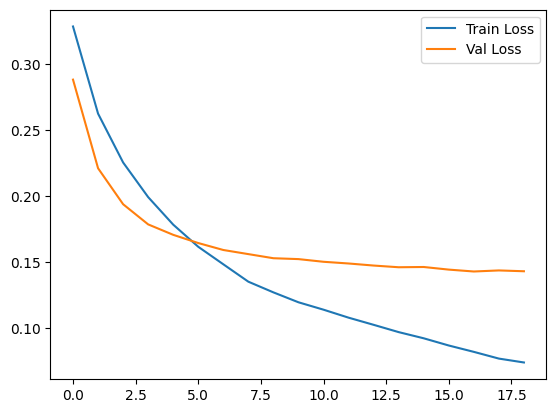
\includegraphics[width=0.75\textwidth]{resim2.png}
    \caption{Overfit}
    \label{fig:my_pic}
\end{figure}


\subsection{(2 Puan)} \textbf{Beşinci soruya ait tüm kodların ve cevapların olduğu jupyter notebook'un Github linkini aşağıdaki url'e koyun.}

\url{https://github.com/melishurkan/Soru5}

\section{(Toplam 10 Puan)} \textbf{Bir önceki sorudaki Prensesi İyileştir problemindeki yapay sinir ağınıza seçtiğiniz herhangi iki farklı regülarizasyon yöntemi ekleyin ve aşağıdaki soruları cevaplayın.} 

\subsection{(2 puan)} \textbf{Kodlarda regülarizasyon eklediğiniz kısımları aşağı koyun:} 

\begin{python}
model = MLP()

lambda_l1 = 0.001  # l1 regülarizasyon katsayısı
optimizer = optim.SGD(model.parameters(), lr=0.01, weight_decay=lambda_l1, momentum=0.8) #l1 regülarizasyonunu optimizer'a ekleme
criterion = nn.BCELoss()
torch.manual_seed(190401079)


train_losses, val_losses = [], []
num_epochs = 1000
batch_size = 16

for epoch in range(num_epochs):
    for i in range(0, len(train_inputs), batch_size):
        batch_inputs = train_inputs[i:i + batch_size]
        batch_targets = train_targets[i:i + batch_size]

        optimizer.zero_grad()
        outputs = model(batch_inputs).squeeze()
        loss = criterion(outputs, batch_targets)
        loss.backward()
        optimizer.step()

    with torch.no_grad():
        train_outputs = model(train_inputs).squeeze()
        train_loss = criterion(train_outputs, train_targets)
        train_losses.append(train_loss.item())

        val_outputs = model(val_inputs).squeeze()
        val_loss = criterion(val_outputs, val_targets)
        val_losses.append(val_loss.item())

        train_predictions = (model(train_inputs) > 0.5).float()
        test_predictions = (model(test_inputs) > 0.5).float()
        val_predictions = (model(val_inputs) > 0.5).float()

    if epoch > 10 and val_losses[-1] > val_losses[-3]:
        break

    if epoch % 1 == 0:
        print(f"Epoch {epoch} | Train Loss: {train_loss:.5f} | Val Loss: {val_loss:.5f}")

test_outputs = model(test_inputs).squeeze()
test_loss = criterion(test_outputs, test_targets)
test_acc = ((test_outputs > 0.5).float() == test_targets).float().mean()

print(f"Test Loss: {test_loss:.5f} | Test Acc: {test_acc:.5f}")
\end{python}

\subsection{(2 puan)} \textbf{Test setinden yeni accuracy, F1, precision ve recall değerlerini hesaplayıp aşağı koyun:}

Epoch 0 | Train Loss: 0.48716 | Val Loss: 0.41180

Epoch 1 | Train Loss: 0.22081 | Val Loss: 0.19686

Epoch 2 | Train Loss: 0.15801 | Val Loss: 0.15695

Epoch 3 | Train Loss: 0.17003 | Val Loss: 0.17312

Epoch 4 | Train Loss: 0.20052 | Val Loss: 0.21356

Epoch 5 | Train Loss: 0.17138 | Val Loss: 0.18364

Epoch 6 | Train Loss: 0.15913 | Val Loss: 0.17646

Epoch 7 | Train Loss: 0.11589 | Val Loss: 0.14034

Epoch 8 | Train Loss: 0.10647 | Val Loss: 0.14254

Epoch 9 | Train Loss: 0.09220 | Val Loss: 0.15164

Epoch 10 | Train Loss: 0.07498 | Val Loss: 0.15306

Test Loss: 0.14210 | Test Acc: 0.95466

Train:F1 Score: 0.97115 | Accuracy: 0.97125 | Recall: 0.98217 | Precision: 0.96038

Test:F1 Score: 0.95460 | Accuracy: 0.95466 | Recall: 0.94845 | Precision: 0.96084

Val:F1 Score: 0.94704 | Accuracy: 0.94586 | Recall: 0.97436 | Precision: 0.92121

\subsection{(5 puan)} \textbf{Regülarizasyon yöntemi seçimlerinizin sebeplerini ve sonuçlara etkisini yorumlayın:}

Early stopping ve L1 regülarizasyon yöntemlerini kullandım. L1 regülarizasyon yöntemini eklemeden önce sadece early stopping kullanarak 25 epoch çıktı alıyordum ancak L1 regülarizasyon yöntemini ekledikten sonra 10 epoch çıktı aldım ve test accuary 0.94171'den 0.95466'ya yükseldi. Test veri setinin F1,accuary ve recall değerlerinde artış gözlemlendi.Cpu'da çalışma zamanı 4.5 saniyeden 0.72 saniye'ye düştü.

\subsection{(1 puan)} \textbf{Sonucun github linkini  aşağıya koyun:}

\url{https://github.com/melishurkan/Soru6}

\end{document}